\bta{动量和动量定理}

\begin{enumerate}[leftmargin=0em]
\renewcommand{\labelenumi}{\arabic{enumi}.}
% A(\Alph) a(\alph) I(\Roman) i(\roman) 1(\arabic)
%设定全局标号series=example	%引用全局变量resume=example
%[topsep=-0.3em,parsep=-0.3em,itemsep=-0.3em,partopsep=-0.3em]
%可使用leftmargin调整列表环境左边的空白长度 [leftmargin=0em]
\item
\exwhere{$ 2012 $年天津卷}
\begin{enumerate}
\renewcommand{\labelenumi}{\arabic{enumi}.}
% A(\Alph) a(\alph) I(\Roman) i(\roman) 1(\arabic)
%设定全局标号series=example	%引用全局变量resume=example
%[topsep=-0.3em,parsep=-0.3em,itemsep=-0.3em,partopsep=-0.3em]
%可使用leftmargin调整列表环境左边的空白长度 [leftmargin=0em]
\item
质量为$ 0.2 \ kg $的小球竖直向下以$ 6 \ m/s $的速度落至水平地面,再以$ 4 \ m/s $的速度反向弹回,取竖直向上为正方向,则小球与地面碰撞前后的动量变化为 \tk{2} $ kg \cdot \ m/s $。
\item 
若小球与地面的作用时间为$ 0.2 \ s $,则小球受到地面的平均作用力大小为 \tk{12} $ N $($ g=10 \ m/s ^{2} $)。



\end{enumerate}

\item 
\exwhere{$ 2014 $年物理上海卷}
动能相等的两物体$ A $、$ B $在光滑水平面上沿同一直线相向而行,它们的速度大小之比
$ v_{A} $∶$ v_{B} $ $ =2: $ $ 1 $,则动量大小之比$ P_{A} $∶$ P_{B} = $ \tk{$ 1:2 $} ;两者碰后粘在一起运动,其总动量与$ A $原来动量大小之比$ P $∶$ P_{A} = $ \tk{$ 1:1 $} 。


\item 
\exwhere{$ 2017 $年海南卷}
光滑水平桌面上有$ P $、$ Q $两个物块,$ Q $的质量是$ P $的$ n $倍。将一轻弹簧置于$ P $、$ Q $之间,用外力缓慢压$ P $、$ Q $。撤去外力后,$ P $、$ Q $开始运动,$ P $和$ Q $的动量大小的比值为 \xzanswer{D} 
\fourchoices
{$ n^{2} $}
{$ n $}
{$ \frac{1}{n} $}
{$ 1 $}




\item
\exwhere{$ 2015 $年理综重庆卷}
高空作业须系安全带。如果质量为$ m $的高空作业人员不慎跌落,从开始跌落到安全带对人刚产生作用力前人下落的距离为$ h $(可视为自由落体运动)。.此后经历时间$ t $安全带达到最大伸长,若在此过程中该作用力始终竖直向上。则该段时间安全带对人的平均作用力大小为 \xzanswer{A} 

\fourchoices
{$\frac { m \sqrt { 2 g h } } { t } + m g \quad$}
{$\frac { m \sqrt { 2 g h } } { t } - m g \quad$}
{$\frac { m \sqrt { g h } } { t } + m g \quad$}
{$\frac { m \sqrt { g h } } { t } - m g$}


\item
\exwhere{$ 2015 $年理综北京卷}
“蹦极”运动中,长弹性绳的一端固定,另一端绑在人身上,人从几十米高处跳下,将蹦极过程简化为人沿竖直方向的运动。从绳恰好伸直,到人第一次下降至最低点的过程中,下列分析正确的是 \xzanswer{A} 

\fourchoices
{绳对人的冲量始终向上,人的动量先增大后减小}
{绳对人的拉力始终做负功,人的动能一直减小}
{绳恰好伸直时,绳的弹性势能为零,人的动能最大}
{人在最低点时,绳对人的拉力等于人所受的重力}



\item
\exwhere{$ 2018 $年全国\lmd{2}卷}
高空坠物极易对行人造成伤害。若一个$ 50 $ $ g $的鸡蛋从一居民楼的$ 25 $层坠下,与地面的撞击时间约为$ 2 $ $ ms $,则该鸡蛋对地面产生的冲击力约为 \xzanswer{C} 

\fourchoices
{$ 10 $ $ N $}
{$ 10^2 $ $ N $	}
{$ 10^3 $ $ N $	 }
{$ 10^4 $ $ N $}

\item 
\exwhere{$ 2018 $年北京卷}
$ 2022 $年将在我国举办第二十四届冬奥会,跳台滑雪是其中最具观赏性的项目之一。某滑道示意图如下,长直助滑道$ AB $与弯曲滑道$ BC $平滑衔接,滑道$ BC $高$ h $ $ = $ $ 10 $ $ m $,$ C $是半径$ R $ $ = $ $ 20 $ $ m $圆弧的最低点。质量$ m $ $ = $ $ 60 $ $ kg $的运动员从$ A $处由静止开始匀加速下滑,加速度$ a $ $ = $ $ 4.5 $ $ m/s^{2} $,到达$ B $点时速度$ v_{B} $ $ = $ $ 30 $ $ m/s $。取重力加速度$ g=10\ m/s^{2} $。
\begin{enumerate}
\renewcommand{\labelenumi}{\arabic{enumi}.}
% A(\Alph) a(\alph) I(\Roman) i(\roman) 1(\arabic)
%设定全局标号series=example	%引用全局变量resume=example
%[topsep=-0.3em,parsep=-0.3em,itemsep=-0.3em,partopsep=-0.3em]
%可使用leftmargin调整列表环境左边的空白长度 [leftmargin=0em]
\item
求长直助滑道$ AB $的长度$ L $;
\item 
求运动员在$ AB $段所受合外力的冲量$ I $的大小;
\item 
若不计$ BC $段的阻力,画出运动员经过$ C $点时的受力图,并求其所受支持力$ F_{N} $的大小。

\end{enumerate}
\begin{figure}[h!]
\flushright
\includesvg[width=0.25\linewidth]{picture/svg/509}
\end{figure}

\banswer{
\begin{enumerate}
\renewcommand{\labelenumi}{\arabic{enumi}.}
% A(\Alph) a(\alph) I(\Roman) i(\roman) 1(\arabic)
%设定全局标号series=example	%引用全局变量resume=example
%[topsep=-0.3em,parsep=-0.3em,itemsep=-0.3em,partopsep=-0.3em]
%可使用leftmargin调整列表环境左边的空白长度 [leftmargin=0em]
\item
$L = \frac { v _ { B } ^ { 2 } - v _ { A } ^ { 2 } } { 2 a } = 100 \mathrm { m }$
\item 
$I = m v _ { B } - m v _ { A } = 1800 \mathrm { N } \cdot \mathrm { s }$
\item 
$F _ { \mathrm { N } } - m g = m \frac { v _ { C } ^ { 2 } } { R }$,得$F _ { N } = 3900 \mathrm { N }$。


\end{enumerate}


}


\item 
\exwhere{$ 2013 $年天津卷}
我国女子短道速滑队在今年世锦赛上实现女子$ 3000 \ m $接力三连冠。观察发现,“接棒”的运动员甲提前站在“交捧”的运动员乙前面,并且开始向前滑行,待乙追上甲时,乙猛推甲一把,使甲获得更大的速度向前冲出。在乙推甲的过程中,忽略运动员与冰面间在水平方向上的相互作用,则 \xzanswer{B} 
\begin{figure}[h!]
\centering
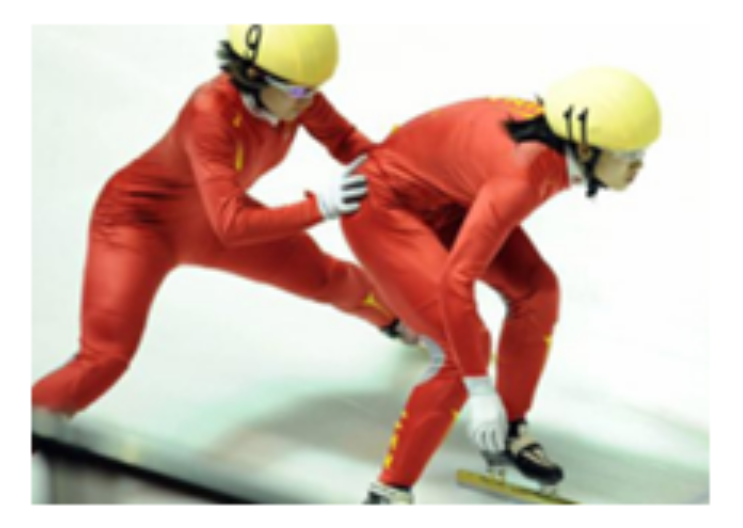
\includegraphics[width=0.3\linewidth]{picture/screenshot002}
\end{figure}



\fourchoices
{甲对乙的冲量一定等于乙对甲的冲量}
{甲、乙的动量变化一定大小相等方向相反}
{甲的动能增加量一定等于乙的动能减少量}
{甲对乙做多少负功,乙对甲就一定做多少正功}



\item 
\exwhere{$ 2017 $年新课标$ \lmd{3} $卷}
一质量为$ 2 $ $ kg $的物块在合外力$ F $的作用下从静止开始沿直线运动。$ F $随时间$ t $变化的图线如图所示,则 \xzanswer{	AB} 
\begin{figure}[h!]
\centering
\includesvg[width=0.23\linewidth]{picture/svg/510}
\end{figure}

\fourchoices
{$ t=1 $ $ s $时物块的速率为$ 1 $ $ m/s $}
{$ t=2 $ $ s $时物块的动量大小为$ 4 $ $ kg \cdot m/s $}
{$ t=3 $ $ s $时物块的动量大小为$ 5 $ $ kg \cdot m/s $}
{$ t=4 $ $ s $时物块的速度为零}


\item
\exwhere{$ 2013 $年天津卷}	
$ 10 $.($ 16 $分)质量为$ m=4 \ kg $的小物块静止于水平地面上的$ A $点,现用$ F=10 \ N $的水平恒力拉动物块一段时间后撤去,物块继续滑动一段位移停在$ B $点,$ A $、$ B $两点相距$ x=20m $,物块与地面间的动摩擦因数$ \mu =0.2 $,$ g $取$ 10 \ m/s^{2} $,求:
\begin{enumerate}
\renewcommand{\labelenumi}{\arabic{enumi}.}
% A(\Alph) a(\alph) I(\Roman) i(\roman) 1(\arabic)
%设定全局标号series=example	%引用全局变量resume=example
%[topsep=-0.3em,parsep=-0.3em,itemsep=-0.3em,partopsep=-0.3em]
%可使用leftmargin调整列表环境左边的空白长度 [leftmargin=0em]
\item
物块在力$ F $作用过程发生位移$ x_{1} $的大小;
\item 
撤去力$ F $后物块继续滑动的时间$ t $。


\end{enumerate}

\banswer{
\begin{enumerate}
\renewcommand{\labelenumi}{\arabic{enumi}.}
% A(\Alph) a(\alph) I(\Roman) i(\roman) 1(\arabic)
%设定全局标号series=example	%引用全局变量resume=example
%[topsep=-0.3em,parsep=-0.3em,itemsep=-0.3em,partopsep=-0.3em]
%可使用leftmargin调整列表环境左边的空白长度 [leftmargin=0em]
\item
$ x_{1}=16\ m $

\item 
$ t=2\ s $

\end{enumerate}


}



\item 
\exwhere{$ 2015 $年理综天津卷}
某快递公司分拣邮件的水平传输装置示意如图,皮带在电动机的带动下保持$ v=1 \ m/s $的恒定速度向右运动,现将一质量为$ m=2 \ kg $的邮件轻放在皮带上,邮件和皮带间的动摩擦因数$ \mu =0.5 $,设皮带足够长,取$ g=10 \ m/s^{2} $,在邮件与皮带发生相对滑动的过程中,求:
\begin{enumerate}
\renewcommand{\labelenumi}{\arabic{enumi}.}
% A(\Alph) a(\alph) I(\Roman) i(\roman) 1(\arabic)
%设定全局标号series=example	%引用全局变量resume=example
%[topsep=-0.3em,parsep=-0.3em,itemsep=-0.3em,partopsep=-0.3em]
%可使用leftmargin调整列表环境左边的空白长度 [leftmargin=0em]
\item
邮件滑动的时间$ t $;
\item 
邮件对地的位移大小$ x $;
\item 
邮件与皮带间的摩擦力对皮带做的功$ W $.

\end{enumerate}
\begin{figure}[h!]
\flushright
\includesvg[width=0.25\linewidth]{picture/svg/511}
\end{figure}

\banswer{
\begin{enumerate}
\renewcommand{\labelenumi}{\arabic{enumi}.}
% A(\Alph) a(\alph) I(\Roman) i(\roman) 1(\arabic)
%设定全局标号series=example	%引用全局变量resume=example
%[topsep=-0.3em,parsep=-0.3em,itemsep=-0.3em,partopsep=-0.3em]
%可使用leftmargin调整列表环境左边的空白长度 [leftmargin=0em]
\item
$ 0.2\ s $
\item 
$ 0.1\ m $
\item 
$ -2\ J $

\end{enumerate}


}


\newpage
\item 
\exwhere{$ 2015 $年理综安徽卷}
一质量为$ 0.5 $ $ kg $的小物块放在水平地面上的$ A $点,距离$ A $点$ 5 $ $ m $的位置$ B $处是一面墙,如图所示。物块以$ v_{0} =9 $ $ m/s $的初速度从$ A $点沿$ AB $方向运动,在与墙壁碰撞前瞬间的速度为$ 7 $ $ m/s $,碰后以$ 6 $ $ m/s $的速度反向运动直至静止。$ g $取$ 10 $ $ m/s^{2} $。
\begin{enumerate}
\renewcommand{\labelenumi}{\arabic{enumi}.}
% A(\Alph) a(\alph) I(\Roman) i(\roman) 1(\arabic)
%设定全局标号series=example	%引用全局变量resume=example
%[topsep=-0.3em,parsep=-0.3em,itemsep=-0.3em,partopsep=-0.3em]
%可使用leftmargin调整列表环境左边的空白长度 [leftmargin=0em]
\item
求物块与地面间的动摩擦因数$ \mu $;
\item 
若碰撞时间为$ 0.05 $ $ s $,求碰撞过程中墙面对物块平均作用力的大小$ F $;
\item 
求物块在反向运动过程中克服摩擦力所做的功$ W $。



\end{enumerate}
\begin{figure}[h!]
\flushright
\includesvg[width=0.35\linewidth]{picture/svg/512}
\end{figure}


\banswer{
\begin{enumerate}
\renewcommand{\labelenumi}{\arabic{enumi}.}
% A(\Alph) a(\alph) I(\Roman) i(\roman) 1(\arabic)
%设定全局标号series=example	%引用全局变量resume=example
%[topsep=-0.3em,parsep=-0.3em,itemsep=-0.3em,partopsep=-0.3em]
%可使用leftmargin调整列表环境左边的空白长度 [leftmargin=0em]
\item
$ 0.32 $
\item 
$ 130\ N $
\item 
$ 9\ J $

\end{enumerate}


}



\item 
\exwhere{$ 2016 $年北京卷}
如图所示,一颗人造卫星原来在椭圆轨道$ 1 $绕地球$ E $运行,在$ P $变轨后进入轨道$ 2 $做匀速圆周运动。下列说法正确的是 \xzanswer{B} 
\begin{figure}[h!]
\centering
\includesvg[width=0.17\linewidth]{picture/svg/513}
\end{figure}

\fourchoices
{不论在轨道$ 1 $还是在轨道$ 2 $运行,卫星在$ P $点的速度都相同}
{不论在轨道$ 1 $还是在轨道$ 2 $运行,卫星在$ P $点的加速度都相同}
{卫星在轨道$ 1 $的任何位置都具有相同加速度}
{卫星在轨道$ 2 $的任何位置都具有相同动量}


\newpage
\item 
\exwhere{$ 2016 $年北京卷}

\begin{enumerate}
\renewcommand{\labelenumi}{\arabic{enumi}.}
% A(\Alph) a(\alph) I(\Roman) i(\roman) 1(\arabic)
%设定全局标号series=example	%引用全局变量resume=example
%[topsep=-0.3em,parsep=-0.3em,itemsep=-0.3em,partopsep=-0.3em]
%可使用leftmargin调整列表环境左边的空白长度 [leftmargin=0em]
\item
动量定理可以表示为$ \Delta p=F \Delta t $,其中动量$ p $和力$ F $都是矢量。在运用动量定理处理二维问题时,可以在相互垂直的$ x $、$ y $两个方向上分别研究。例如,质量为$ m $的小球斜射到木板上,入射的角度是$ \theta $,碰撞后弹出的角度也是$ \theta $,碰撞前后的速度大小都是$ v $,如图$ 1 $所示。碰撞过程中忽略小球所受重力。
\begin{figure}[h!]
\centering
\includesvg[width=0.25\linewidth]{picture/svg/514}
\end{figure}

$ a $.分别求出碰撞前后$ x $、$ y $方向小球的动量变化$ \Delta p_x $、$ \Delta p_y $;

$ b $.分析说明小球对木板的作用力的方向。

\item 
激光束可以看作是粒子流,其中的粒子以相同的动量沿光传播方向运动。激光照射到物体上,在发生反射、折射和吸收现象的同时,也会对物体产生作用。光镊效应就是一个实例,激光束可以像镊子一样抓住细胞等微小颗粒。
\begin{figure}[h!]
\centering
\includesvg[width=0.23\linewidth]{picture/svg/515}
\end{figure}

一束激光经$ S $点后被分成若干细光束,若不考虑光的反射和吸收,其中光束①和②穿过介质小球的光路如图②所示,图中$ O $点是介质小球的球心,入射时光束①和②与$ SO $的夹角均为$ \theta $,出射时光束均与$ SO $平行。请在下面两种情况下,分析说明两光束因折射对小球产生的合力的方向。

$ a $. 光束①和②强度相同;

$ b $. 光束①比②强度大。 




\end{enumerate}


\banswer{
\begin{enumerate}
\renewcommand{\labelenumi}{\arabic{enumi}.}
% A(\Alph) a(\alph) I(\Roman) i(\roman) 1(\arabic)
%设定全局标号series=example	%引用全局变量resume=example
%[topsep=-0.3em,parsep=-0.3em,itemsep=-0.3em,partopsep=-0.3em]
%可使用leftmargin调整列表环境左边的空白长度 [leftmargin=0em]
\item
a. $\Delta P _ { x } = 0 , \quad \Delta P _ { y } = 2 m v \cos \theta$,方向沿y轴正方向; b. y轴负方向
\item 
a. 两光束对小球的合力的方向沿SO向左 b. 两光束对小球的合力的方向指向左上方


\end{enumerate}


}




\item 
\exwhere{$ 2019 $年物理全国\lmd{1}卷}
最近,我国为“长征九号”研制的大推力新型火箭发动机联试成功,这标志着我国重型运载火箭的研发取得突破性进展。若某次实验中该发动机向后喷射的气体速度约为$ 3 $ $ km/s $,产生的推力约为$ 4.8 \times 108 $ $ N $,则它在$ 1 $ $ s $时间内喷射的气体质量约为 \xzanswer{B} 

\fourchoices
{$ 1.6 \times 10^2 $ $ kg $}
{$ 1.6 \times 10^3 $ $ kg $	}
{$ 1.6 \times 10^5 $ $ kg $ }
{$ 1.6 \times 10^6 $ $ kg $}










\end{enumerate}



